\chapter{Robocup Feature Extraction Techniques}
\label{sec:realtimeFeatureExtraction}

\section{BRISK0 - UBRISK}
\label{sec:brisk0}
In order to make the BRISK algorithm suitable for the Robocup domain, some slight modifications had to be made to the original algorithm. These changes include combining a detector defined as BRISK0, which is a slight variation of the original BRISK implementation, with a variety of Descriptors which will be described below. These feature extraction algorithms are applied to a gray-scale image and matching is performed using Hamming distance as described in \secref{sec:matching}.\\

\subsection{Image Processing}
\label{sec:imageProcessingBrisk}
In the Robocup scenario, when observing features, the robot's head will be tilted upwards at the maximum possible angle in order to observe features that are on or near the ceiling. This is because in a real Robocup environment, dynamic objects such as humans will generate volatile features. These feature are not necessarily repeatable and will potentially hinder the robot's localisation ability.\\

In order to improve the chances of generating non-volatile features, only the section of the image above the robot's horizon line is evaluated. This will effectively remove the dynamic background clutter that is found below the horizon line. In addition to the advantage of generating potentially non-volatile features, evaluating only a sub-section of the image results in a significant increase in computational performance. \\ 

The image processing procedure used for the BRISK-based implementations is as follows. Initially a $640 \times 480$ YUV image captured by the Nao is converted to a gray scale image as shown in \figref{fig:colourGrayscale}. One of the main reasons for this is that it allows the image to be processed along a single channel which optimises computational performance. \\

\begin{figure}[h!] 
  \centering
    \includegraphics[width=0.8\textwidth]{../Drawings/brisk/yuvImageGray.jpg}
    \caption{Conversion of the YUV image captured by the Nao to grayscale}
    \label{fig:colourGrayscale}
\end{figure}

Since we are only interested in features near the ceiling, the bottom section of the image is cropped and remove before image processing begins. This procedure is shown in \figref{fig:cropImage}.\\

\begin{figure}[h!] 
  \centering
    \includegraphics[width=0.8\textwidth]{../Drawings/brisk/croppedImageFromOriginal.jpg}
    \caption{Cropping the gray scale image for processing}
    \label{fig:cropImage}
\end{figure}

\subsection{Detector}
\label{sec:BRISK0Detect}
The BRISK detector typically detects features by progressively half-sampling an image and in doing so creates a scale-space pyramid as defined in \secref{sec:brisk}. Creating this pyramid is computationally expensive but generates robust scale-invariant interest points.\\

The scale-space pyramid is not needed for this application and thus interest points are only detected along a single scale. This is achieved by setting the number of octaves to $0$ on the BRISK detector, effectively creating BRISK0. This causes the scale-space pyramid to be `flattened' to a single layer which is utilised to detect interest points. The effect of this is that FAST scores are only computed for a single layer and thus a non-maximal suppression is only performed on this layer in scale space. This results in a significant increase in computational performance. \\

%In addition to this, more features will be detected as the constraint required for detecting an interest point has been relaxed. This is also useful since regions around the ceiling do not usually have a large amount of variation and thus the amount of interest points detected will be relatively limited.\\

A 2D sub-pixel refinement is still applied to the interest points on the single layer resulting in an increased accuracy in interest point image coordinates.\\

Since only a single octave is utilised and interest points are therefore only detected on a single scale, the 1D parabola that is fitted along the scale-space axis \cite{Leutenegger2011} is also discarded. The disadvantage of this approach is that the local maxima FAST scores are not as accurate as in the original implementation but the increase in accuracy is not crucial in this application as good performance is still obtained as shown in \secref{sec:overallPerformance}. Furthermore, the increase in computational performance is crucial in developing a method that is practically implementable on the robot. This generates a bank of interest points and the descriptors are then computed.\\

\subsection{Descriptor}
\label{sec:BRISK0Describe}
In order to determine the best feature extraction algorithm to be utilised on the robot, a variety of BRISK and SURF descriptors have been combined with the BRISK0 detector. The descriptors include BRISK0, U-BRISK and 2D SURF descriptors respectively.\\

The BRISK0 descriptor complements the BRISK0 detector as assigns the same scale to all of the interest points. This is because interest points are detected on only a single scale as mentioned previously. The rest of the BRISK algorithm is computed according to the original BRISK implementation resulting in a rotation invariant descriptor of length $512$ bits\cite{Leutenegger2011}.\\

The SURF 2D descriptor is also combined with the BRISK0 detector. This creates a descriptor vector of length $64$ as implemented in 2D SURF \cite{Bay}. No modifications have been made to the SURF descriptor resulting in the same output as 2D SURF.\\ 

The U-BRISK descriptor contains a slight modification to the original BRISK descriptor. The rotation of the sampling pattern, which was described in \secref{sec:briskDescribe}, has been discarded. This removes the rotation invariant property of the BRISK feature extraction algorithm, but provides a significant increase in computational performance. The brightness comparison tests used to create the descriptor vector are therefore performed on interest points with a sampling pattern that remains in a standard orientation. The combination of BRISK0 and U-BRISK produces the best overall performance for the Robocup scenario as detailed in \secref{sec:overallPerformance}. \\

\section{1DSURF}
\label{sec:1dsurf}
Another technique that can be utilised for the Robocup is the 1D SURF feature extraction algorithm that has been previously implemented \cite{Anderson} for use in the Robocup. This algorithm extracts features from a single row of pixels in an image $A$. These features are then matched with features extracted from a row of pixels generated from an image $B$ being compared to image $A$. This technique is many orders of magnitude faster than the traditional 2D SURF implementation and is potentially suitable for use in the Robocup \cite{Anderson}.\\

In order to utilise the feature extraction algorithm, it had to be implemented according to the design detailed in \cite{Anderson}. The OpenSURF implementation, which is freely available online \cite{opensurf} has been utilised in order to implement this algorithm.\\

The main task is transforming 2D SURF into its 1D SURF implementation. This requires changes to both the detector and Descriptor and will be explained in the sections to follow.\\

\subsection{Image Processing}
\label{sec:imageProcessing}
The first main step in implementing the 1D SURF algorithm is to extract a single row of gray-scale pixels from the image. This is achieved by sampling every fourth pixel intensity value along the robot's horizon line in order to speed up processing time \cite{Anderson}. 
In addition to this, each sampled pixel intensity value is summed with a vertical band of $30$ pixels as shown in \figref{fig:rows}. This is performed instead of taking the mean primarily since it is faster to compute. This procedure therefore ultimately generates a row of summed pixel intensities. It is from this row of intensities that features will be extracted and matched.\\

\begin{figure}[h!] 
  \centering
    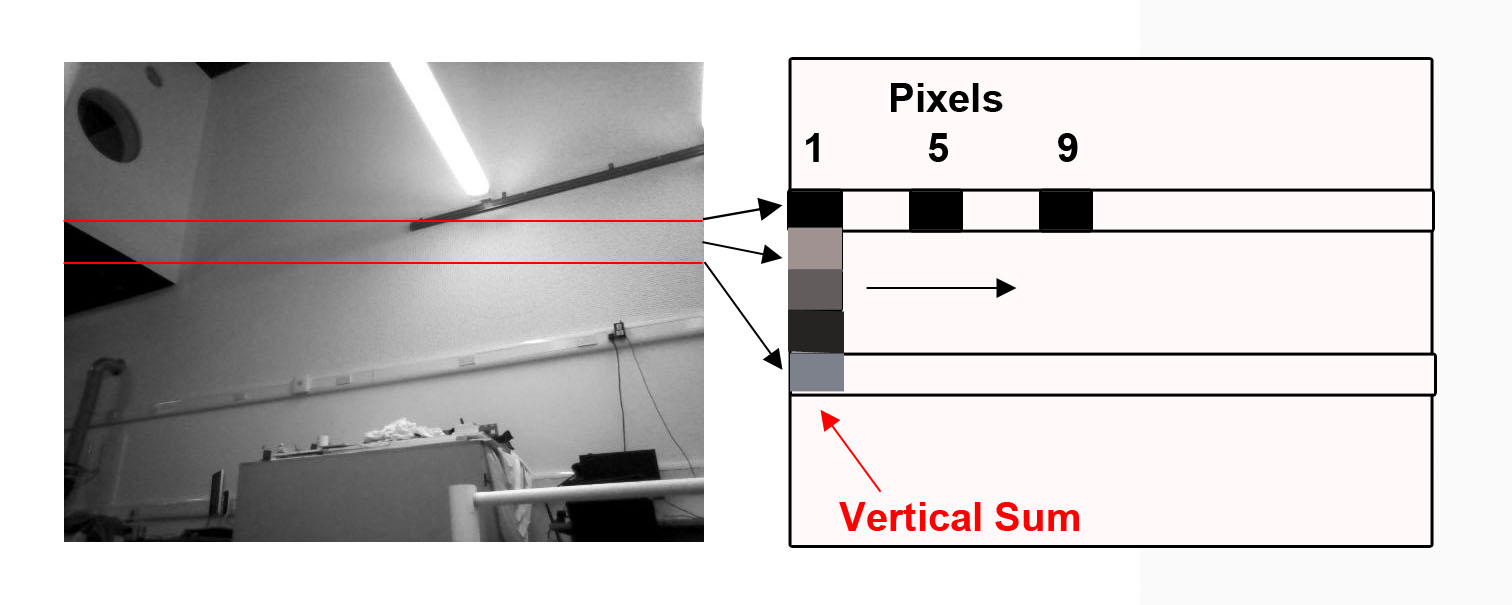
\includegraphics[width=1.0\textwidth]{../Drawings/methods/horizon.jpg}
    \caption{The vertical sum of pixel intensities along a sample horizon line indicated in red. Every fourth pixel is sampled as shown in the right portion of the figure. }
    \label{fig:rows}
\end{figure}

\subsection{Detector}
\label{sec:1dsurfDetect}
The 1D SURF detector has a number of differences from that of its 2D equivalent. The first major difference is the construction of the integral image. The integral image as stated in \secref{sec:integralImages}, allows for fast computation of rectangular areas in an image. Since the image is now 1D, the integral image is only computed along the single row of pixels.\\ 

The next step is calculating the blob response for each point $(x,1)$ along the single row of pixels. In the 2D case, this is typically achieved by performing a 2D convolution, convolving a second order Gaussian derivative with the image at the point $\textbf{x} = (x,y)$. The Gaussian is approximated as a box filter and, combined with the integral image, results in a very efficient computation. In the 1D case, the convolution can only be computed along the single dimensional row of pixels. Thus the box filters have been effectively reduced to 1D box filters and the $xy$ and $y$ directional box filters can be neglected. The determinant of the Hessian can thus be reduced to \eqnref{eqn:reducedHessian}.\\

\begin{equation}
det(Hessian) = D_{xx}D_{xx}
\label{eqn:reducedHessian}
\end{equation} 

The number of octaves chosen for 1D SURF is $4$ and the number of scales per octave is $3$. Once a blob response map has been generated, interest points can be subsequently computed for each octave and each scale within the respective octave. Typically, in order to identify local maxima, each pixel in 3D scale space is compared to its $3 \times 3 \times 3$ surrounding neighbors and a non-maximal suppression is performed \cite{Evans2009}. However, in the case of 1D SURF, this constraint is relaxed and the pixel is only compared to its neighbors in the single scale space dimensional as shown in \figref{fig:singleScale} \cite{Anderson}. The result is that more features will be detected. However, these features will not have as strong responses as the features detected in 2D SURF.\\

\begin{figure}[h!] 
  \centering
    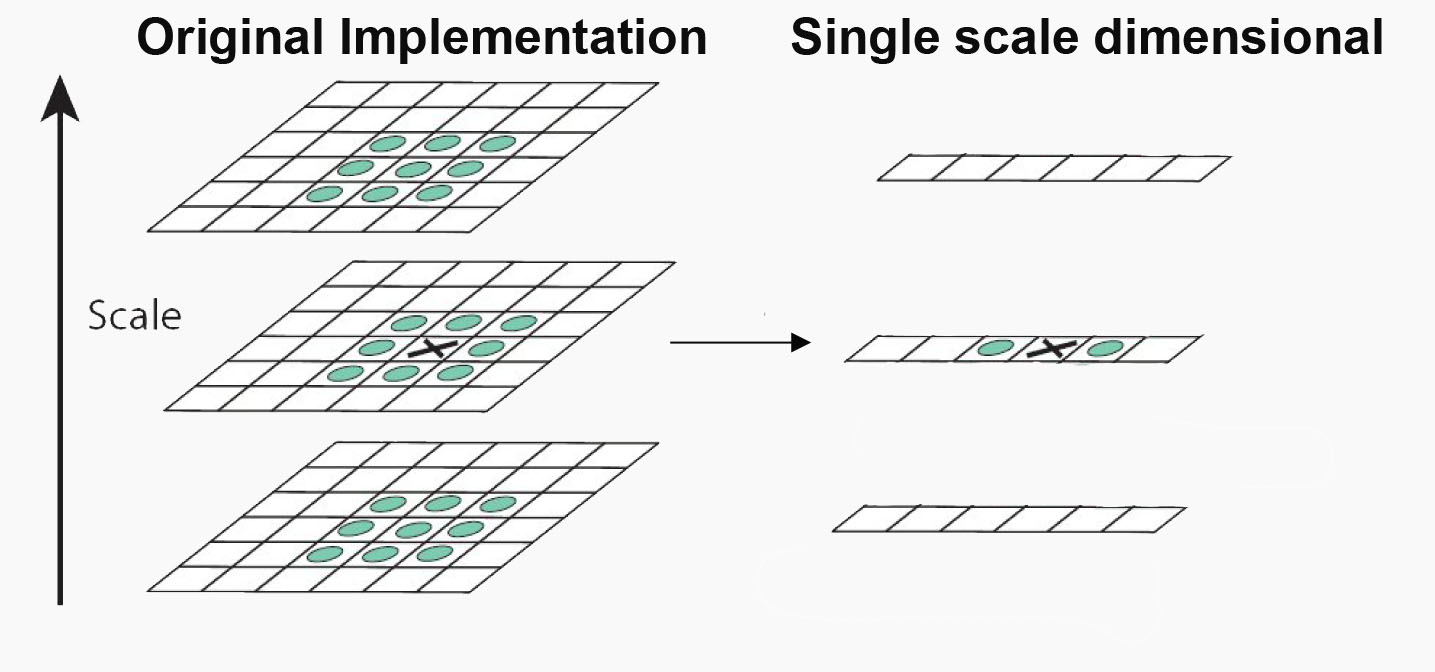
\includegraphics[width=0.8\textwidth]{../Drawings/methods/SURF1D_Nonmaximal_suppression.jpg}
    \caption{1D SURF only uses the single scale dimensional in order to perform non-maximal suppression and detect interest points \cite{Anderson}.}
    \label{fig:singleScale}
\end{figure}

Once this has been achieved, the interest points are usually interpolated in both scale and image space to sub-pixel accuracy \cite{Evans2009}. However, sub-pixel accuracy is not necessary for the Robocup domain and has thus been discarded in the 1D implementation \cite{Anderson}. This procedure ultimately detects a set of interest points along a single row of pixels based on the blob response map. The next step involves computing the descriptors.\\  

\subsection{Descriptor}
\label{sec:1dsurfDescribe}
Typically, the 2D SURF descriptor is constructed in two stages. The first stage involves assigning an orientation to the descriptor and has been described in \secref{sec:2dsurfdescribe}. This step has been discarded since the feature points are assigned with reference to the horizon line and therefore do not require an orientation.\\

In 2D SURF, the second stage involves constructing a square region around the interest point and sub-dividing the region into $16$ equally-sized sub-regions as detailed in \secref{sec:2dsurfdescribe}. For each sub-region, HWRs in both the $x$ and $y$ directions are calculated for $25$ regularly spaced sample points. These responses are summed together to produce $4$ descriptor values for the sub-region corresponding to \eqnref{eqn:descriptorSub}. Therefore, in total a descriptor vector of length $64$ is created.\\

In the case of 1D SURF, it is only possible to utilise $4$ of the $16$ sub-regions along the $x$ direction as shown in \figref{fig:subregions4} due to the reduction in dimensionality of the image. In addition, HWRs can only be calculated along the $x$ direction which allows for the $y$ direction Haar Wavelets to be discarded. The current implementation of 1D SURF further reduces the number of sub-regions to $3$ while still achieving good performance \cite{Anderson}. This will ultimately produce a $6$ dimensional descriptor vector rather than the $64$ dimensional descriptor vector as shown in \eqnref{eqn:descriptor1d}. Each of the $3$ sub-regions will produce a descriptor pair of $[\sum dx_i, \sum |dx_i|]$ where $dx_i$ refers to the HWR from the $i^{th}$ sub-region in the $x$ direction. \\

\begin{figure}[h!] 
  \centering
    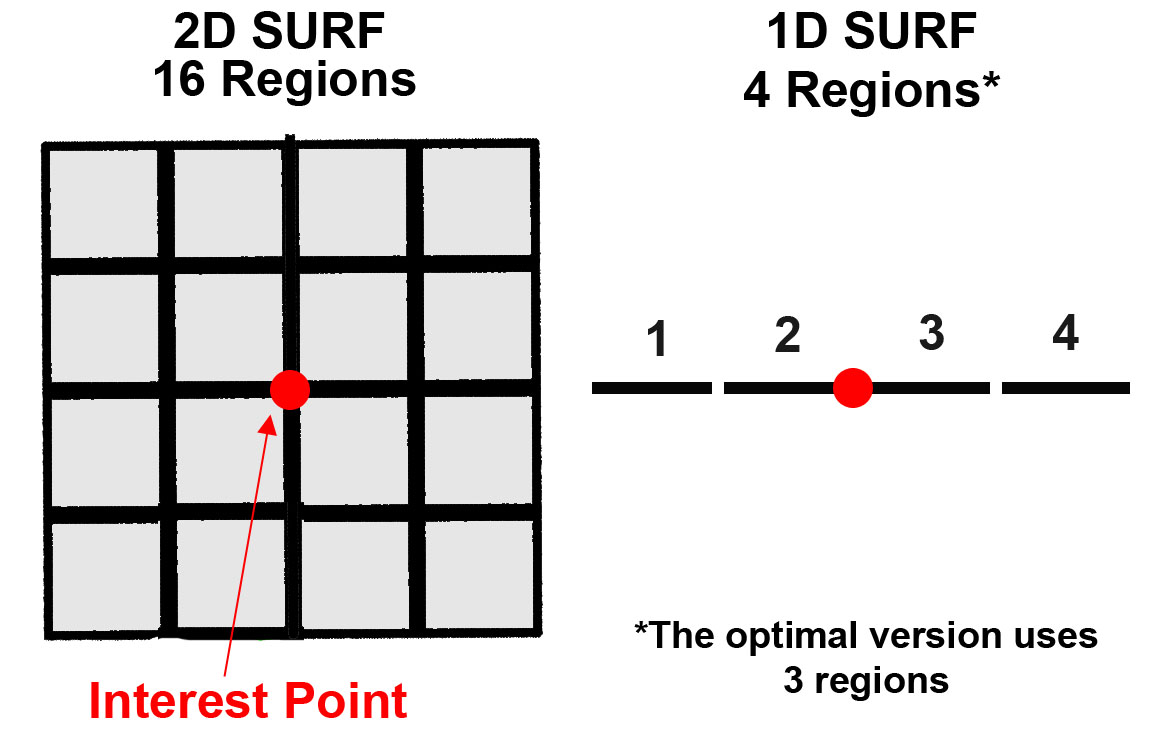
\includegraphics[width=0.5\textwidth]{../Drawings/methods/SURF1D_Descriptor.jpg}
    \caption{Using only 4 sub-regions (3 in the optimal case) to compute the descriptors for each interest point}
    \label{fig:subregions4}
\end{figure}


\begin{equation}
descriptor = [ \sum dx_1, \sum |dx_1|,\sum dx_2, \sum |dx_2|,\sum dx_3, \sum |dx_3|] 
\label{eqn:descriptor1d}
\end{equation}

\section{Summary}
\label{sec:summary3}